
% Croatian Ties chapter -----------------------------------------------
\chapter*{Croatian Ties}
\addcontentsline{toc}{chapter}{Croatian Ties}

\begin{flushright}
\parbox{0.7\textwidth}{
\emph{Secrecy is the first essential in affairs of the State. \\
\hspace*{\fill}{\textperiodcentered \textperiodcentered \textperiodcentered \hspace*{0.2em} De Richelieu} } }
\end{flushright}

\noindent
Croatian Ties is chess variant which is played on 10 x 10 board,
with silver and red fields and dark silver and dark red pieces.
In algebraic notation, columns are enumerated from 'a' to 'j',
and rows are enumerated from '1' to '10'. A new piece is
introduced, Pegasus.

\clearpage

\section*{Pegasus}
\addcontentsline{toc}{section}{Pegasus}

\noindent
\begin{wrapfigure}[9]{l}{0.4\textwidth}
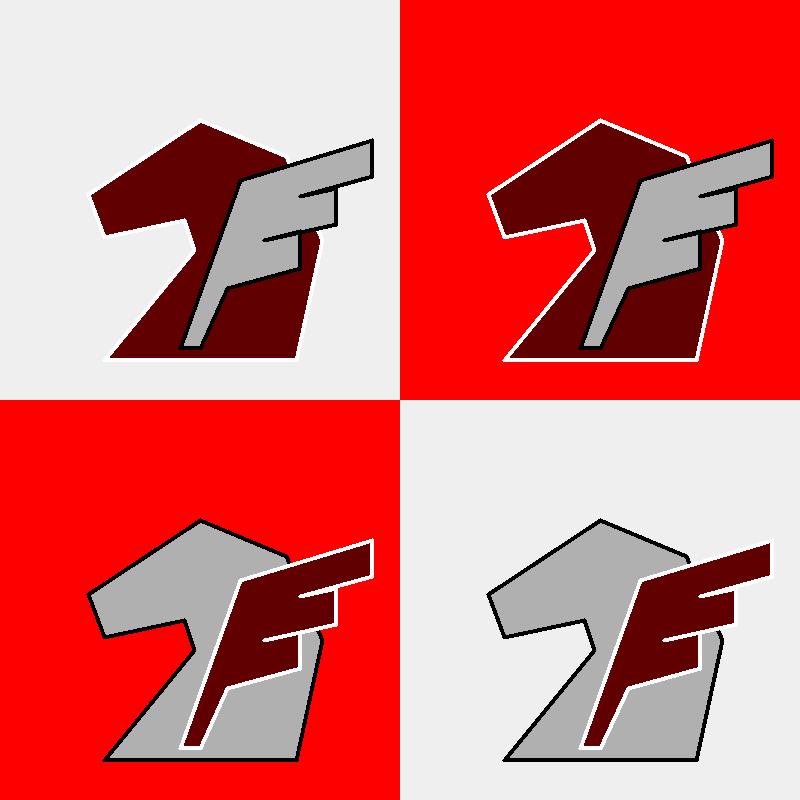
\includegraphics[width=0.4\textwidth, keepaspectratio=true]{pieces/07_pegasus.png}
\caption{Pegasus}
\label{fig:pegasus}
% % \centering
\end{wrapfigure}
Pegasus moves similarly to Knight, but it can continue its jumpy movement
until another piece is encountered, or it runs out of board. Note that once
in movement, Pegasus can not change its' heading.

Pegasus symbol in algebraic notation is 'G', to avoid confusion with Pawn.

\vspace{2\baselineskip}

\noindent
\begin{wrapfigure}[12]{l}{0.5\textwidth}
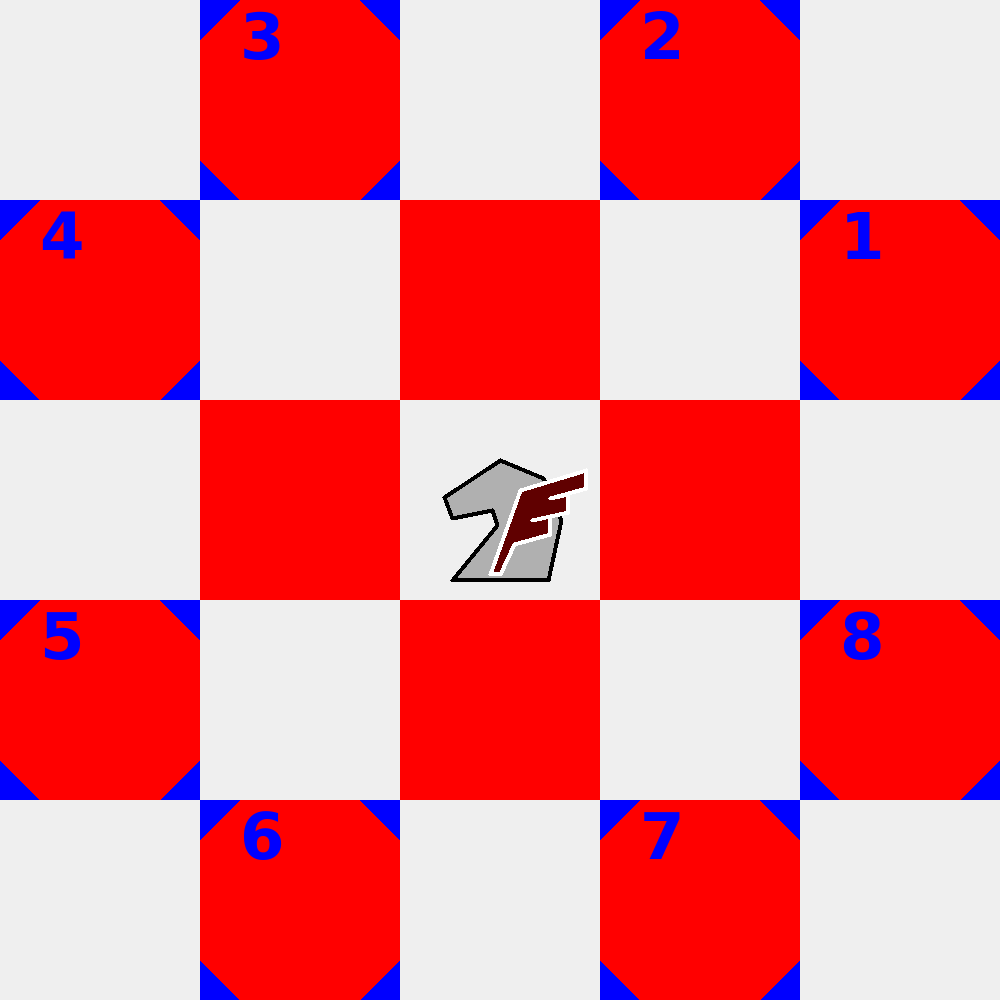
\includegraphics[width=0.5\textwidth, keepaspectratio=true]{examples/01_move_pegasus_initial.png}
\caption{Pegasus initial step}
\label{fig:pegasus_initial_step}
% % \centering
\end{wrapfigure}
In the example on the left we have Pegasus with all valid initial move directions
marked. These all are the same as valid moves for Knight. Pegasus' movement is not
hampered by surrounding piece, if it's placed on any unmarked field. Pegasus can
"jump" over it just as Knight would.

\clearpage

\noindent
% \begin{figure}[t]
\begin{figure}[!t]
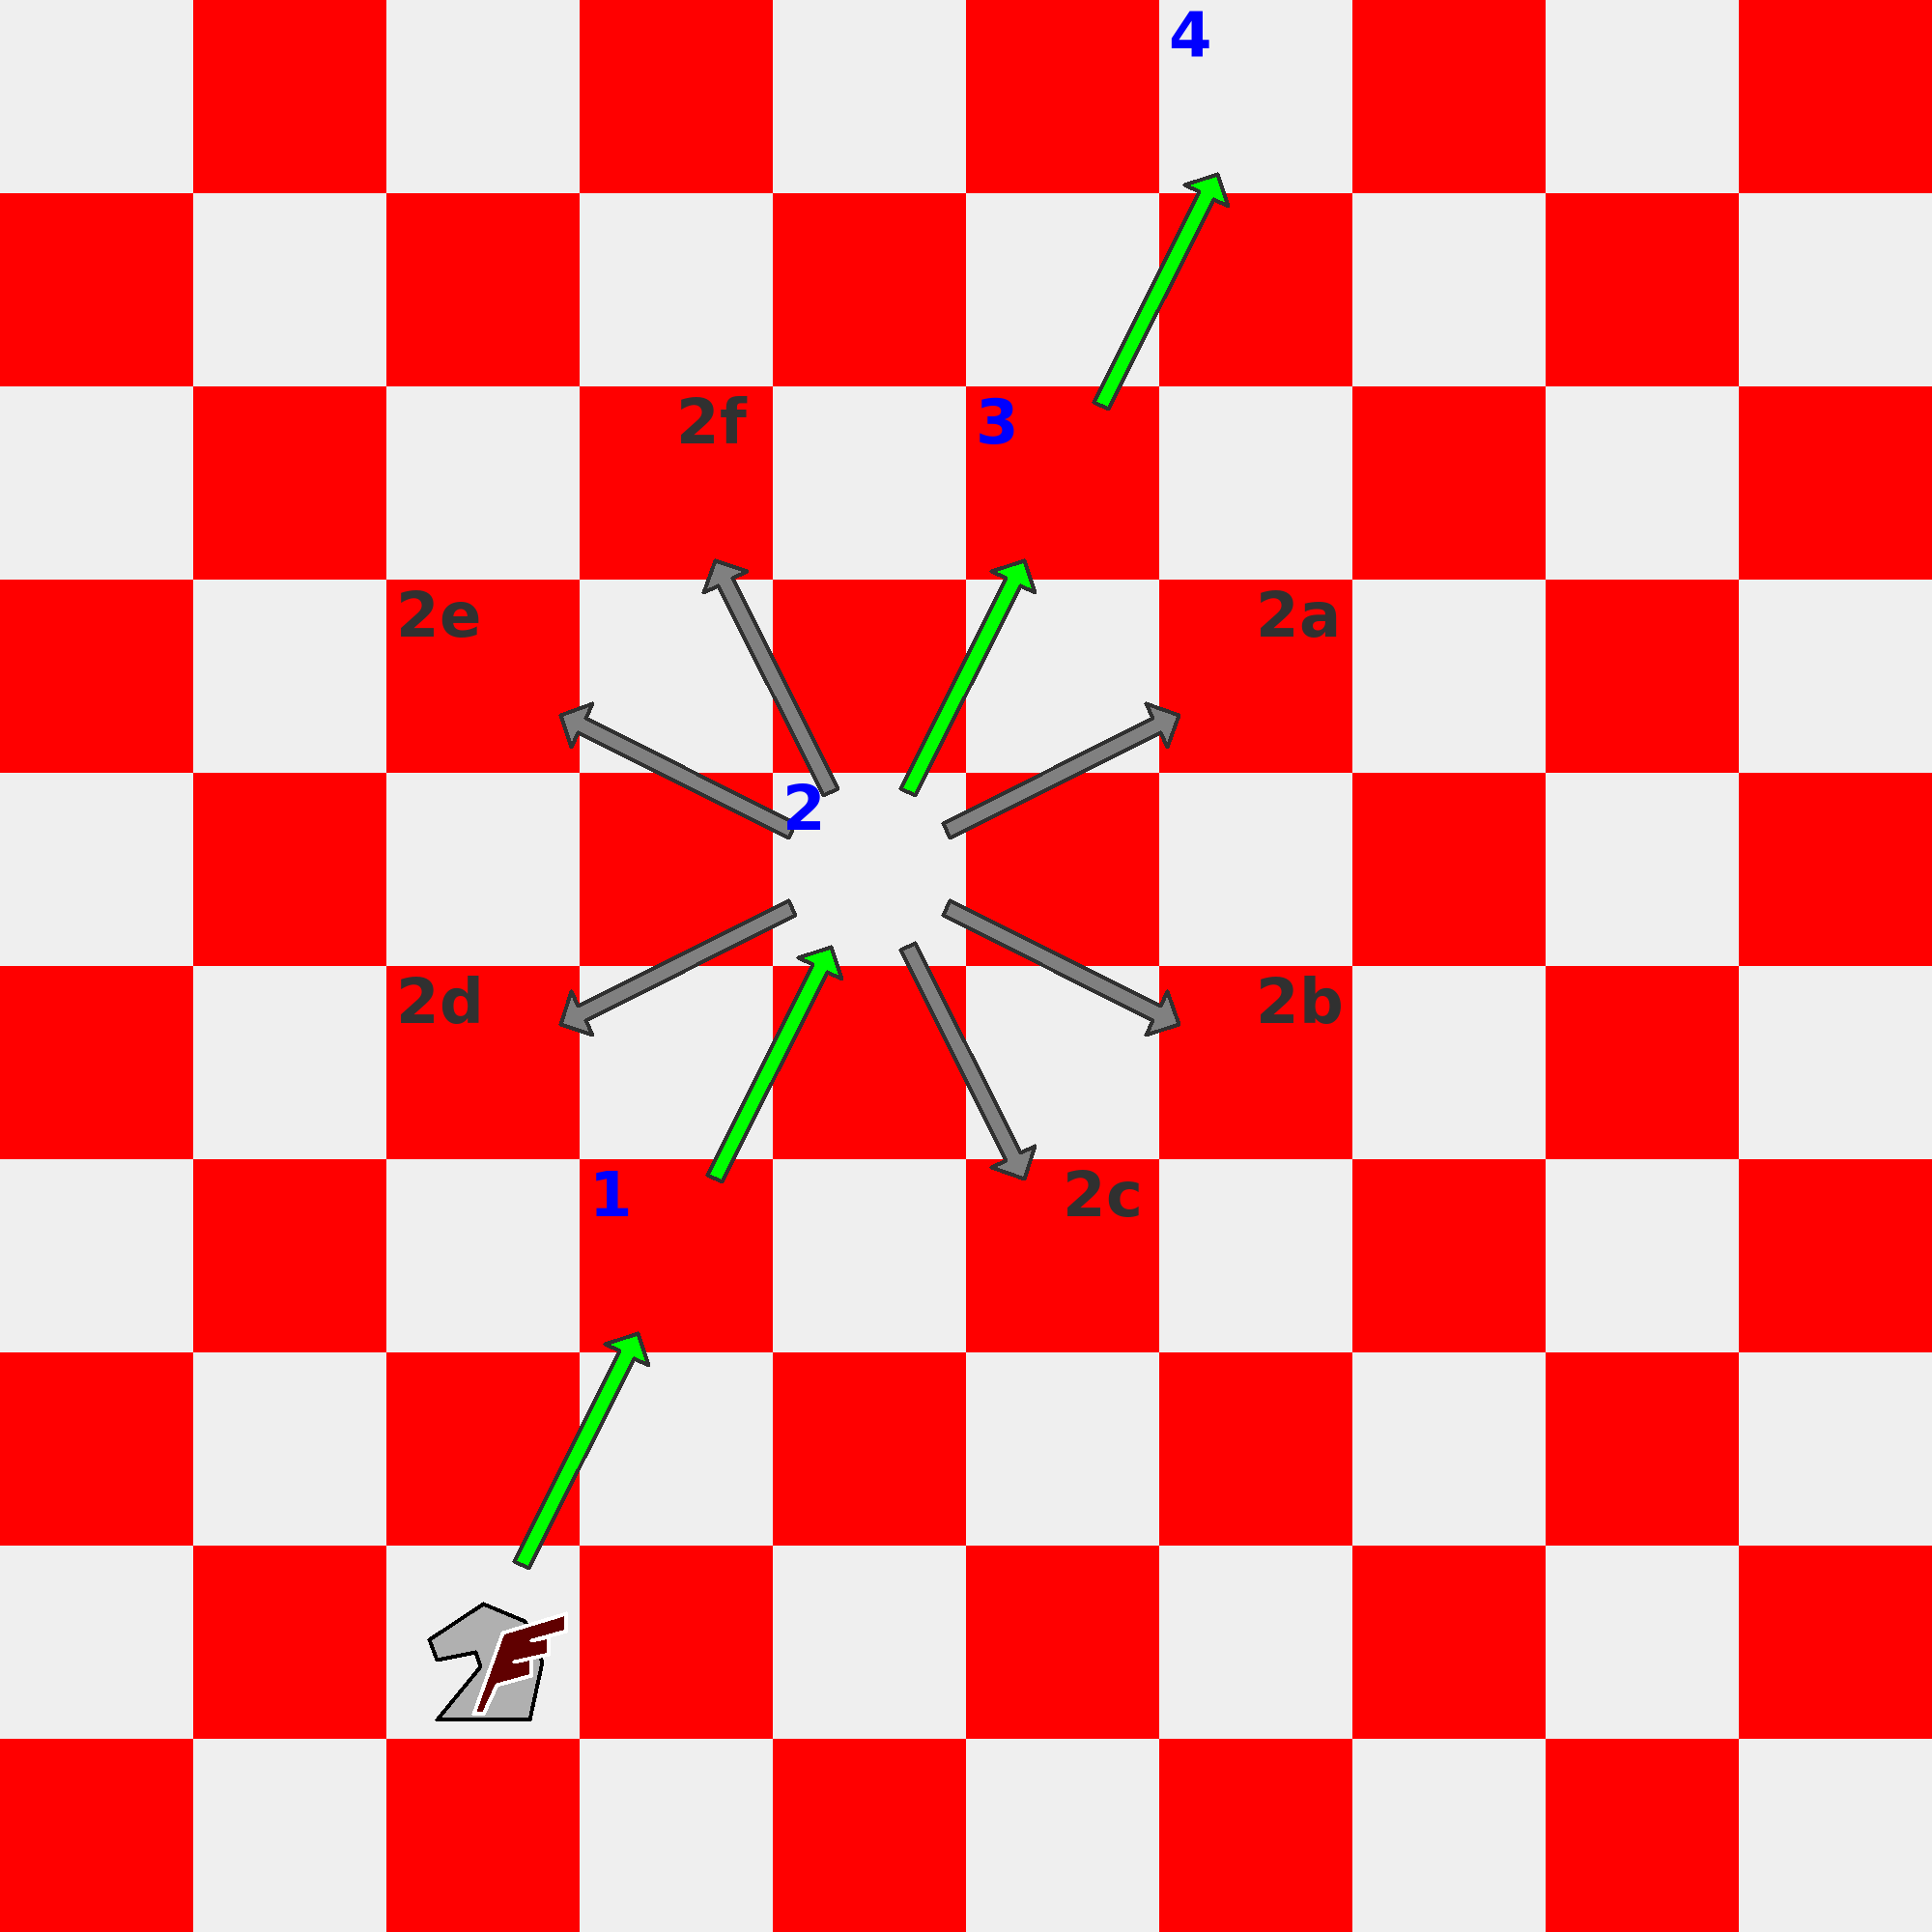
\includegraphics[width=1.0\textwidth, keepaspectratio=true]{examples/02_move_pegasus_direction.png}
\caption{Pegasus move direction}
\label{fig:pegasus_move_direction}
% \centering
\end{figure}
Once direction is chosen Pegasus can continue its' movement performing one jump
after another in order from nearest field to furthest. Here, this is marked
with green arrows. Accessible fields are marked 1 to 4, in order of accessibility,
from nearest to furthest. Again, once direction is chosen it can't be changed
anymore. For instance, after reaching field 2 it's not allowed to change
direction to 2f (or any other greyed-out arrow).

\clearpage

\noindent
% \begin{figure}[t]
\begin{figure}[!t]
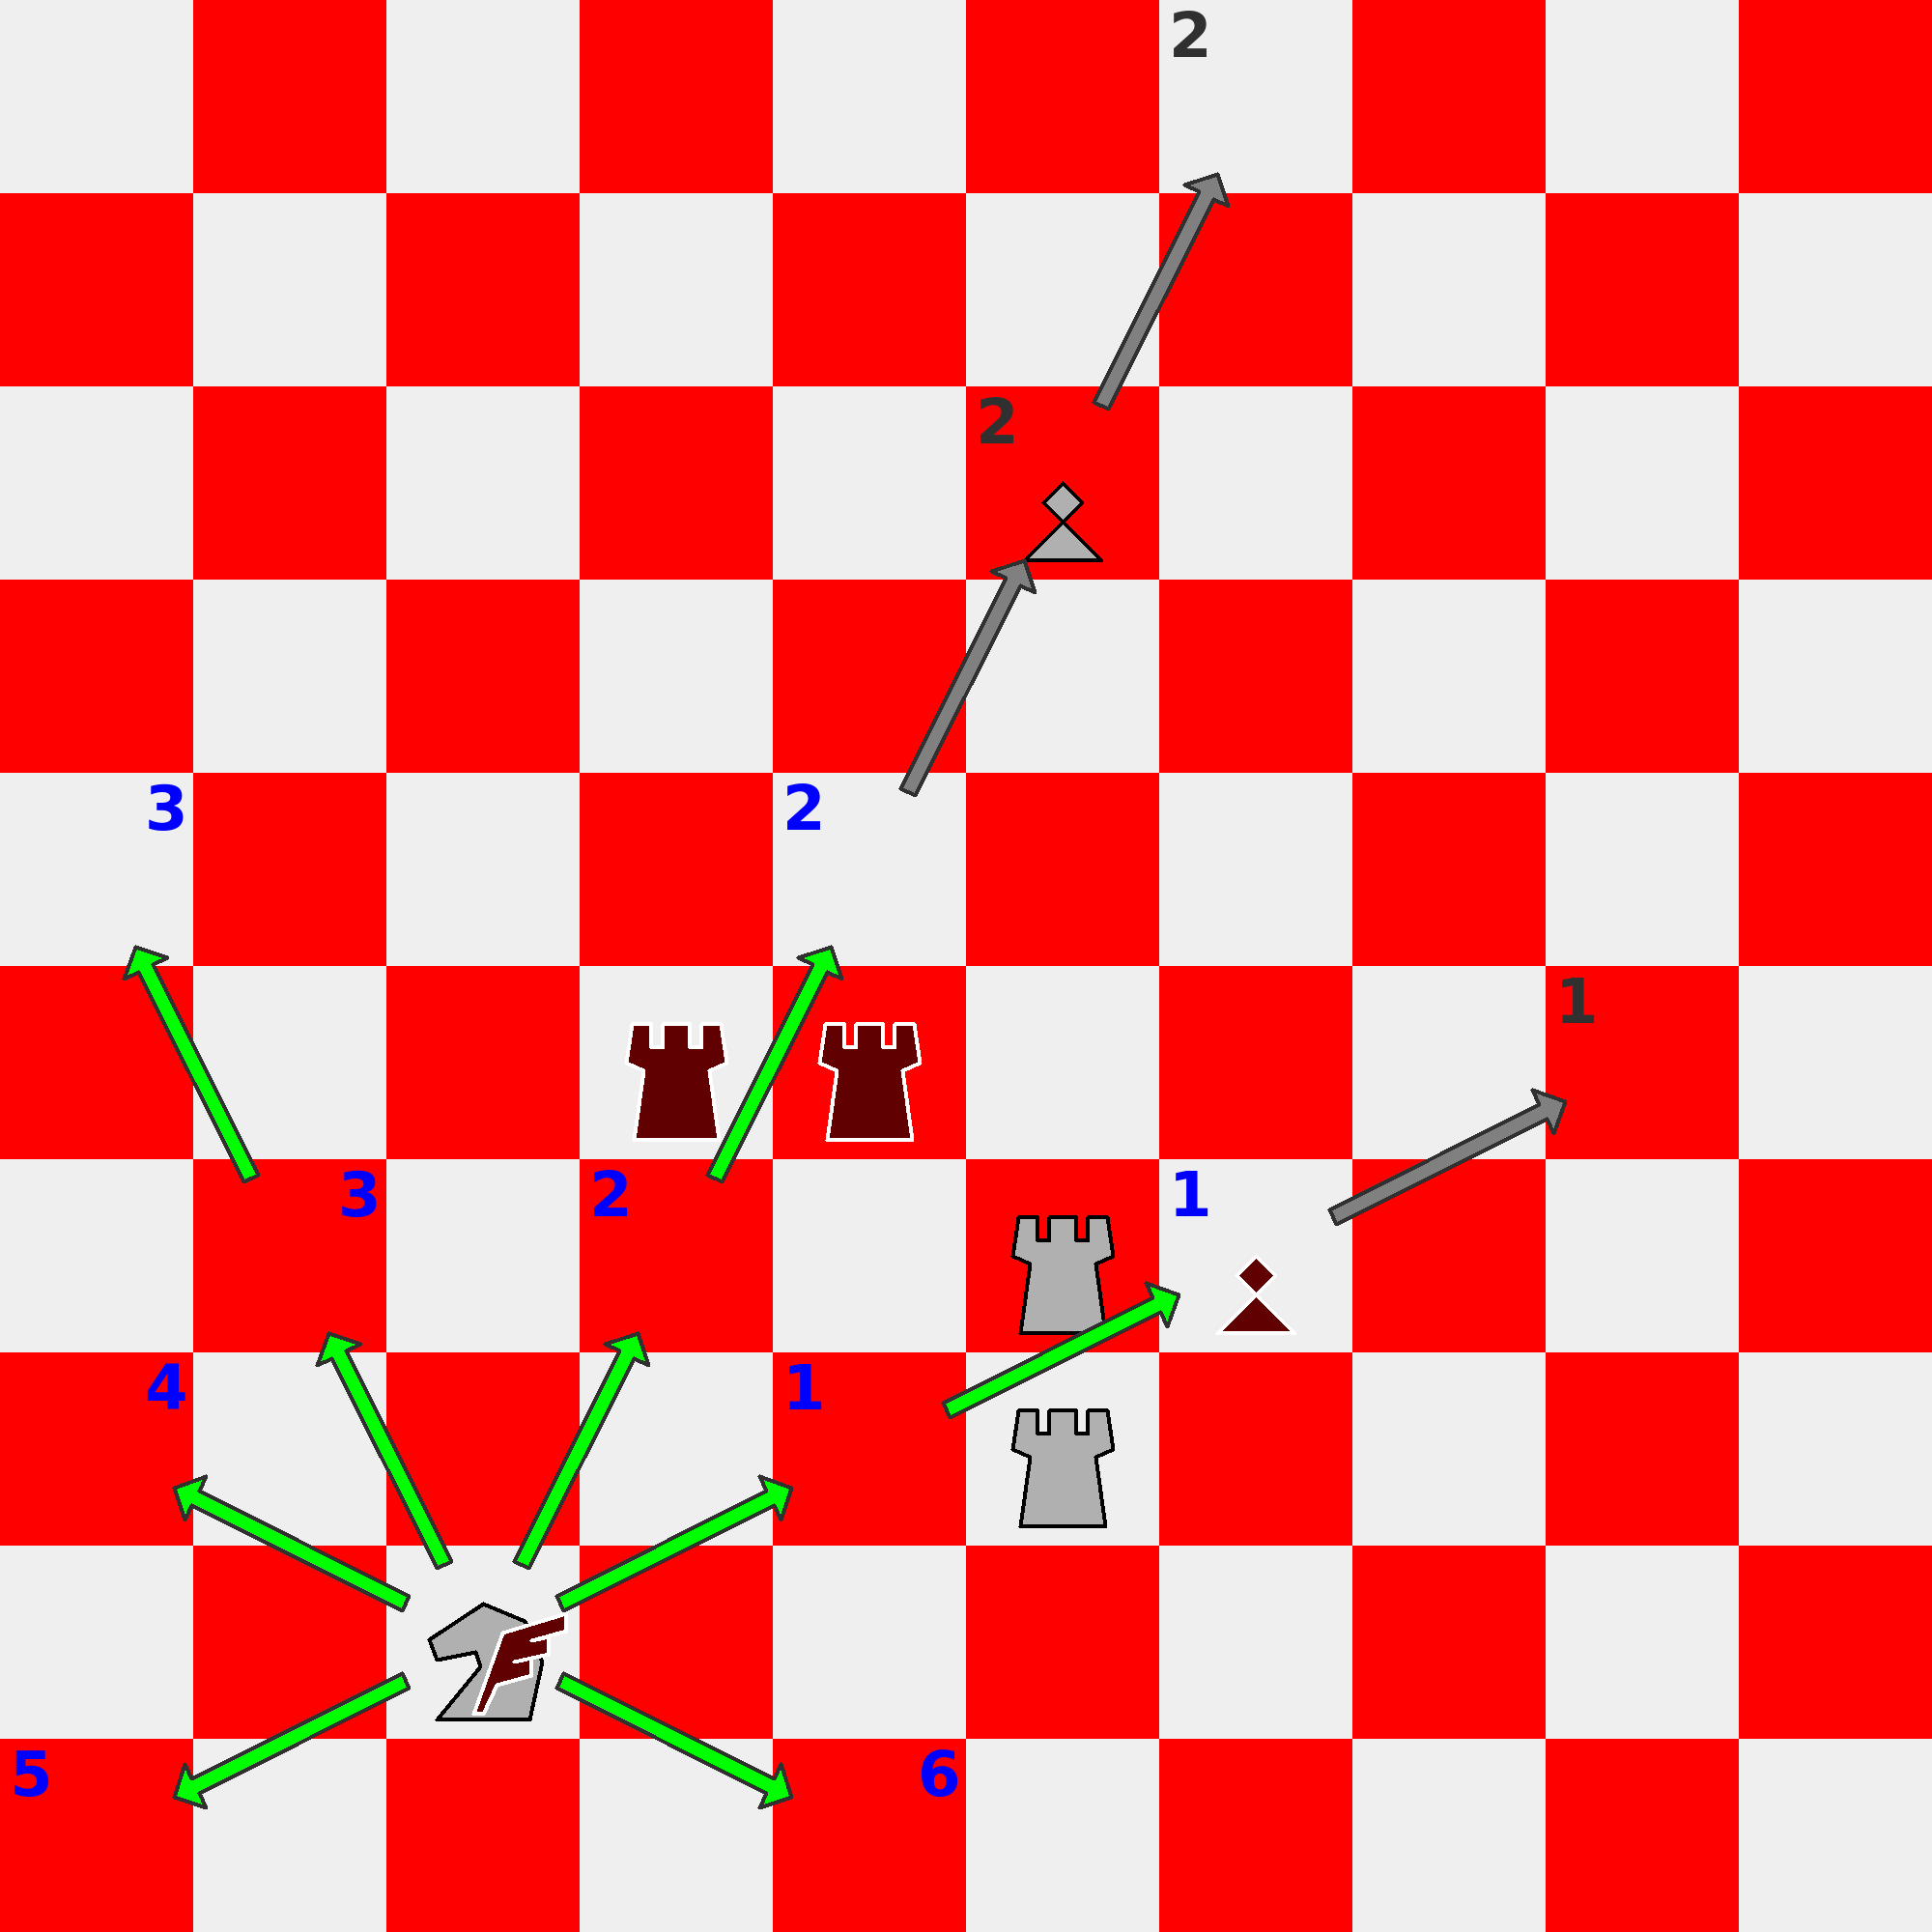
\includegraphics[width=1.0\textwidth, keepaspectratio=true]{examples/03_move_pegasus.png}
\caption{Pegasus moves}
\label{fig:pegasus_moves}
% \centering
\end{figure}
Move along arrow is called step. Field at which arrow points to is called step field.
Pegasus can "jump" over pieces on non-step fields, Rooks in example above. Numbers
here enumerate directions of movement. Own piece on step field stops Pegasus at
preceding step field, see direction 2. Opponent's piece on step field can be captured.
Just as with any other piece that would finish the move, meaning Pegasus would have to
stop at captured step field, see direction 1.

\clearpage

\section*{En passant}
\addcontentsline{toc}{section}{En passant}

\noindent
\begin{wrapfigure}[18]{l}{0.4\textwidth}
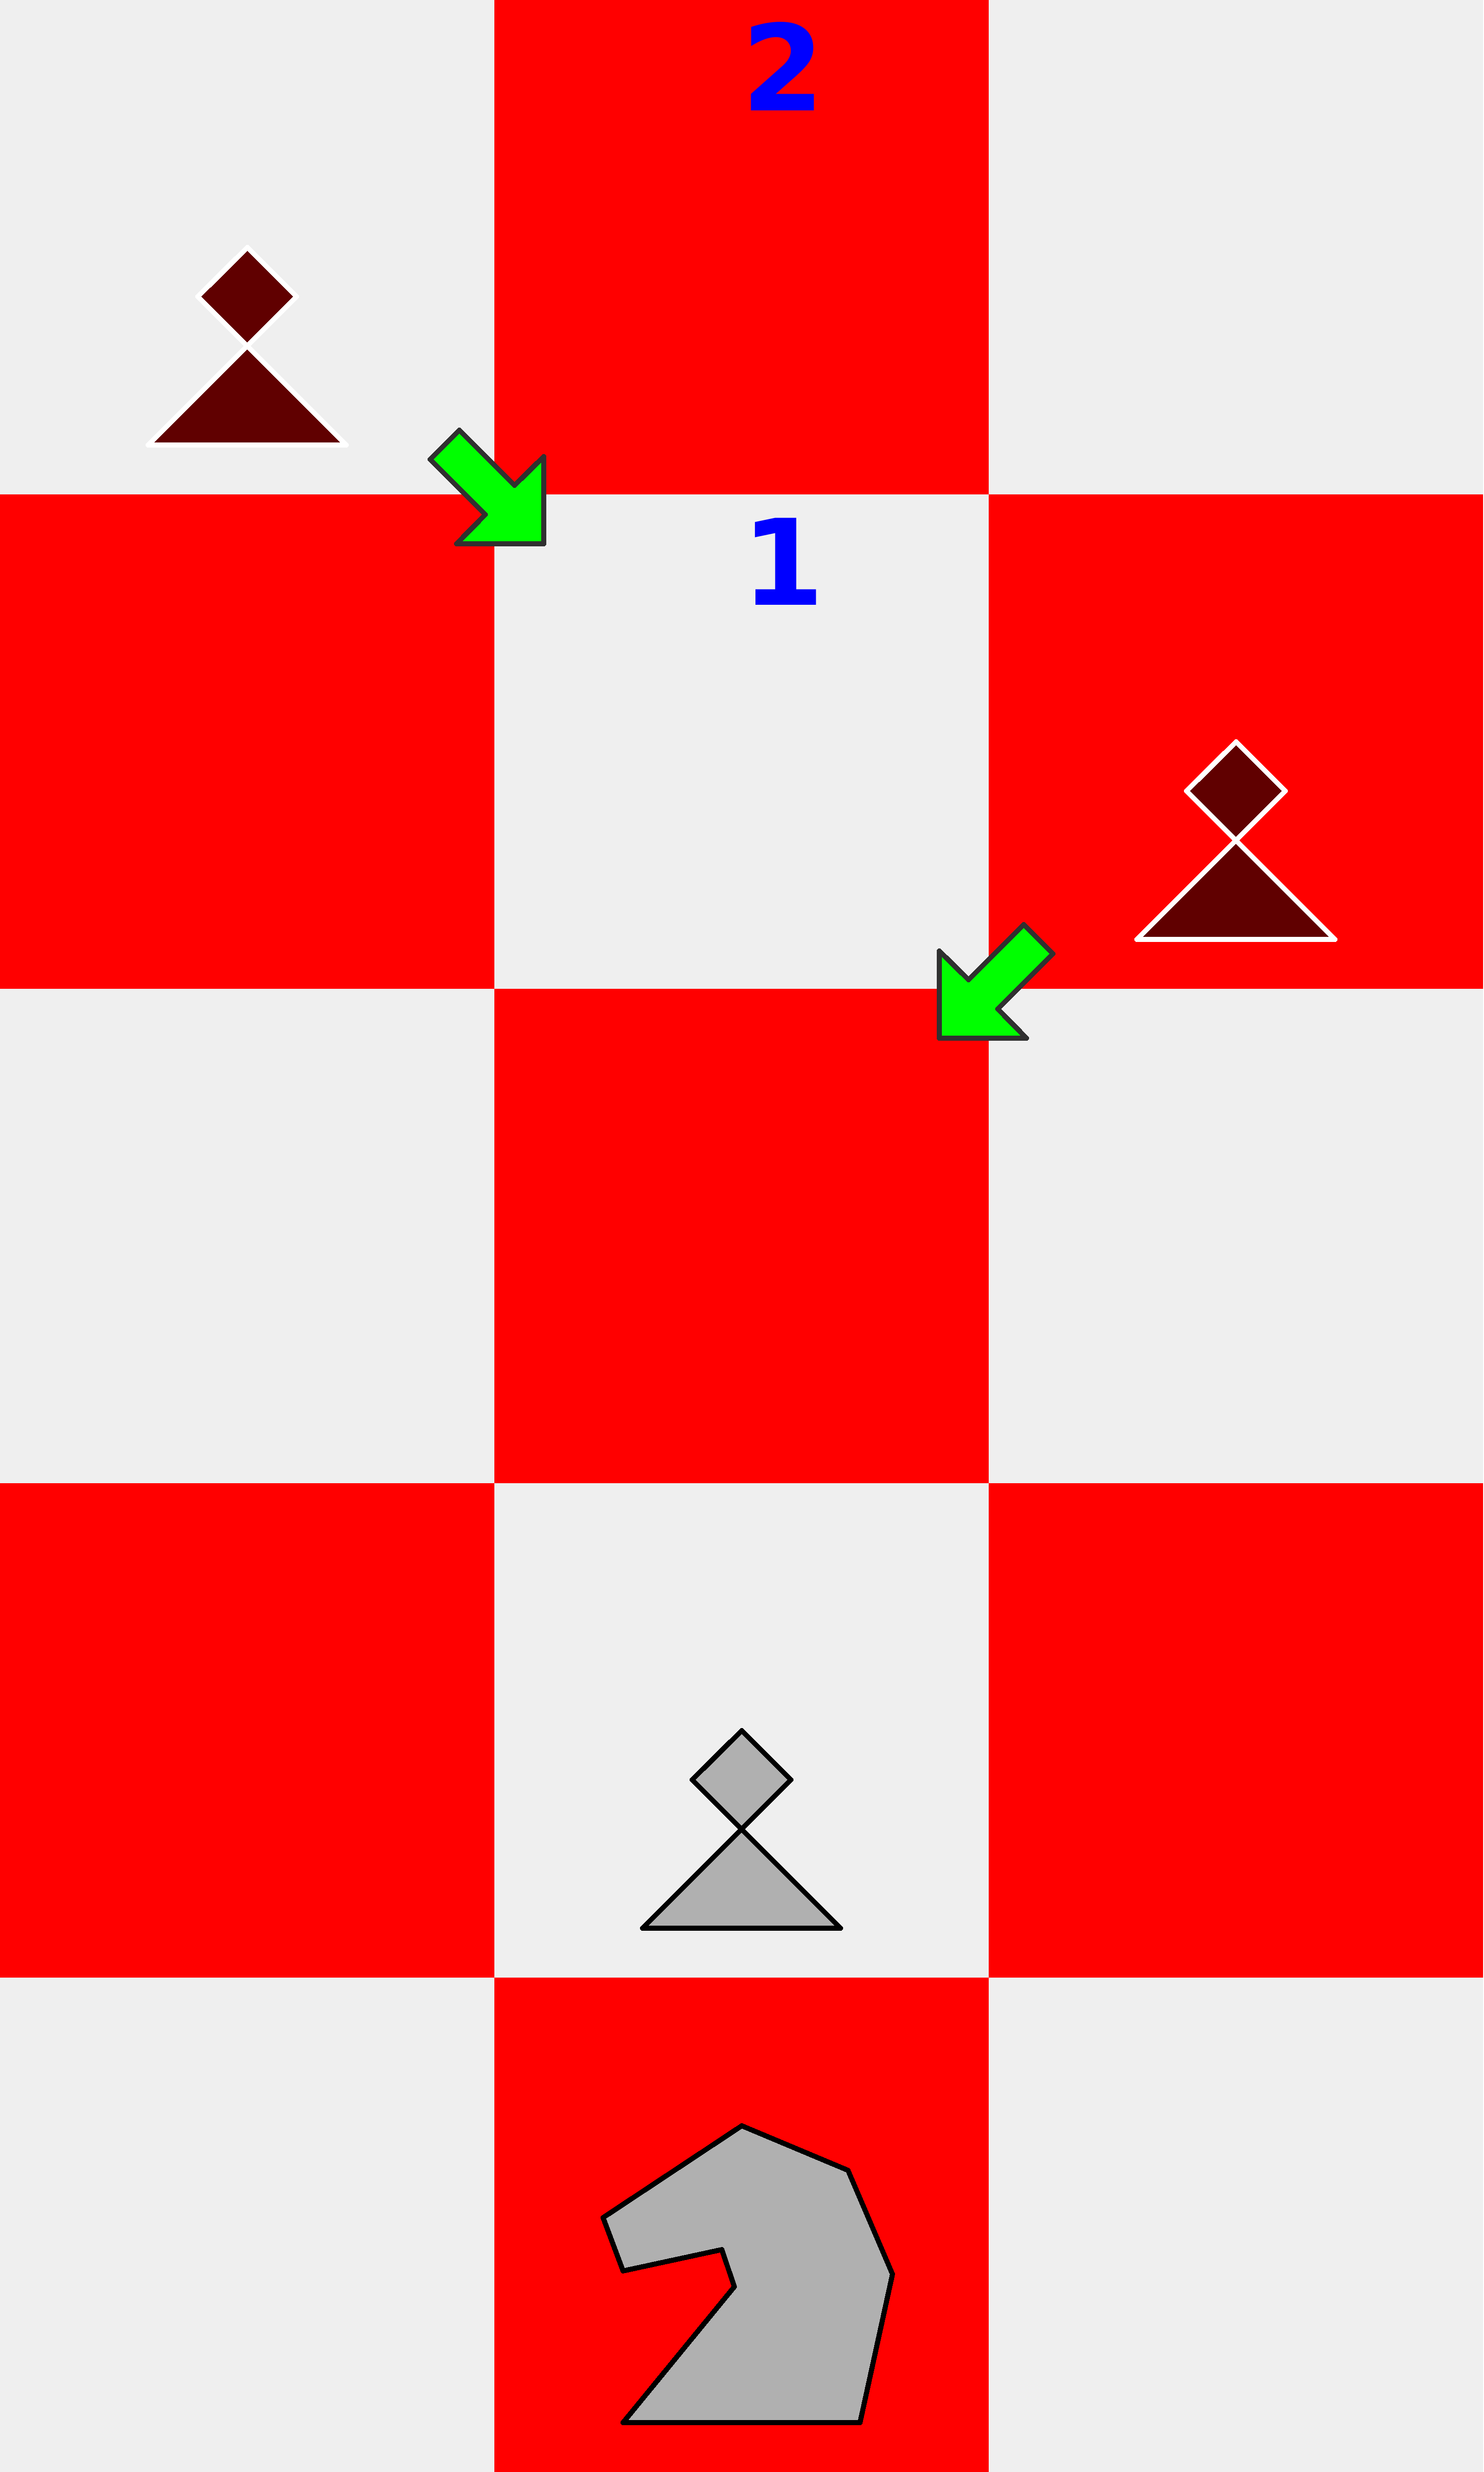
\includegraphics[width=0.4\textwidth, keepaspectratio=true]{en_passants/04_croatian_ties_en_passant.png}
\caption{En passant}
\label{fig:cc_en_passant}
% % \centering
\end{wrapfigure}
En passant is identical to one in Classic Chess, only difference is that Pawn can now
move longer on initial turn, up to 3 fields in this instance. As expected, all passed-by
opponent's Pawns also gain en passant opportunity.

Passed-by opponents are those which are at most at the same row in which Pawn has ended its'
initial move, or which are closer to Pawn's initial position.

In example on left, if light Pawn's initial move was 3 fields long, ending in field marked 2,
both dark Pawns would have en passant opportunity. Naturaly, if initial move was only 2 fields
long, ending in field marked 1, only dark Pawn on the right would gain en passant opportunity.

\clearpage

\section*{Castling}
\addcontentsline{toc}{section}{Castling}

Castling is essentially the same as it is in Classical Chess, only real difference is that
King can move either 2 or 3 fields across. All other constraints from Classical Chess still
applies, described in detail here \\
\href{https://en.wikipedia.org/wiki/Castling}{https://en.wikipedia.org/wiki/Castling}.

\noindent
\begin{figure}[!h]
% \begin{figure}[!t]
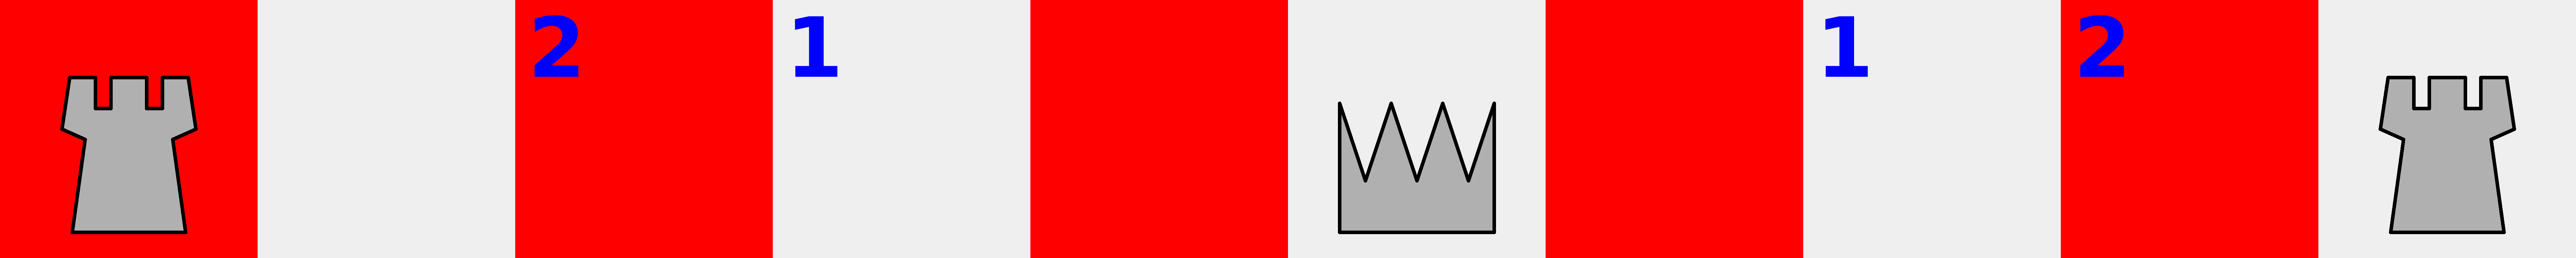
\includegraphics[width=1.0\textwidth, keepaspectratio=true]{castlings/04_croatian_ties_castling.png}
\caption{Castling}
\label{fig:cc_castling}
% \centering
\end{figure}

In example above, all valid King's castling moves are numbered. Regardless if King performs
long or short castling move, Rook would always end up on field next to King, on opposite side
of it, i.e. closer to center.

\noindent
\begin{figure}[!h]
% \begin{figure}[!t]
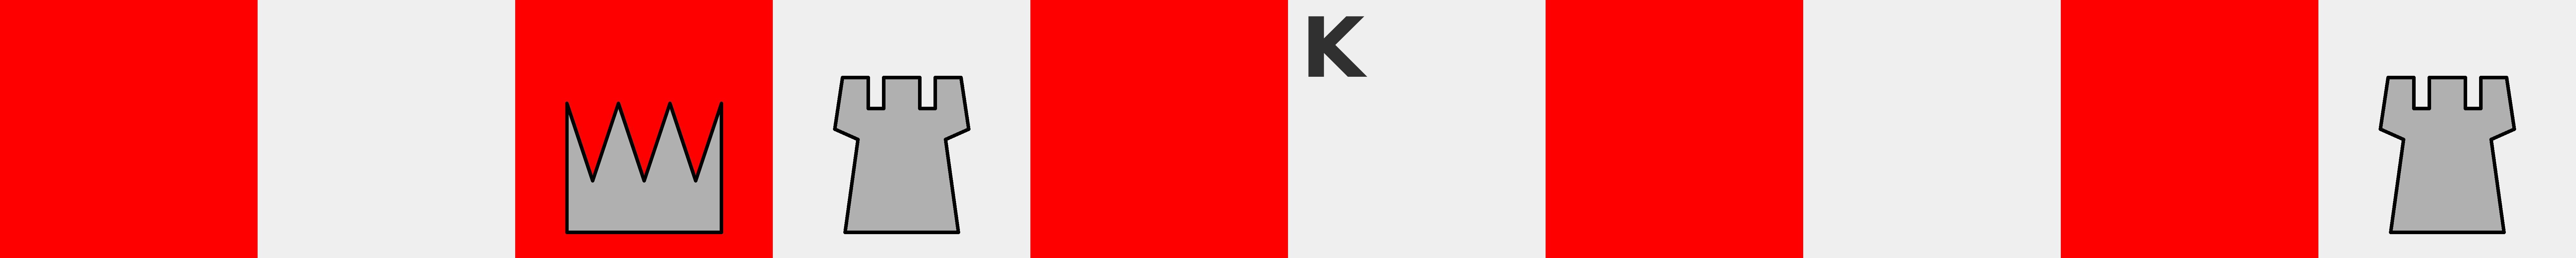
\includegraphics[width=1.0\textwidth, keepaspectratio=true]{castlings/long_left/04_croatian_ties_castling_long_left.png}
\caption{Castling long left}
\label{fig:cc_castling_long_left}
% \centering
\end{figure}

In this example King was castling long to the left. Initial King's position is marked with "K".
After castling is finished, left Rook ends up at field immediately on the right to the King.

\clearpage

\section*{Initial setup}
\addcontentsline{toc}{section}{Initial setup}

Initial setup for Light player is (mirrored for Dark one):
\texttt{PPPPPPPPPP \\
        RGNBQKBNGR}, \\
or more conveniently, as seen in this image:

\noindent
% \begin{figure}[t]
\begin{figure}[h]
\includegraphics[width=1.0\textwidth, keepaspectratio=true]{boards/04_croatian_ties.png}
\caption{Croatian Ties board}
\label{fig:croatian_ties}
% \centering
\end{figure}

\clearpage
% ----------------------------------------------- Croatian Ties chapter
